\documentclass[11pt]{article}
\usepackage{subcaption}
\usepackage{sectsty}
\usepackage{graphicx}
\usepackage{amsmath} % for 'pmatrix' environment
\usepackage{caption}
\usepackage{subcaption}

% Margins
\topmargin=-0.45in
\evensidemargin=0in
\oddsidemargin=0in
\textwidth=6.5in
\textheight=9.0in
\headsep=0.25in

\title{\textbf{Dokumentation zu:\\DRL-Aufgabenblatt "Markov Decision Processes"}}
\author{Erik Viere, Daniel Hilfer, Domenic Scholz}
\date{\today}

\begin{document}
\maketitle	
\pagebreak

\section*{Aufgabe 2.1}
\subsubsection*{a)}
% TODO: Beschreibung Konvergenzverhalten
% TODO: Ergebnisse beschreiben, erklären Auswirkung random Policy

Das Konvergenzverhalten des iterativen Algorithmus zur Bestimmung der State Values ist in Abbildung \ref{img:2_1_a1} und Abbildung \ref{img:2_1_a2} dargestellt. In Abbildung \ref{img:2_1_a1} wird für jede Iteration ermittelt, was die größte Veränderung ist, dabei werden alle Zellen betrachtet. Zu sehen ist, adss bereits nach ca. $6$ Iterationen kaum mehr Veränderungen auftreten. Um eine vollständige Konvergenz sicherzustellen, wurden jedoch insgesamt $15$ Iterationen durchgeführt.\\
\begin{figure}
    \centering
    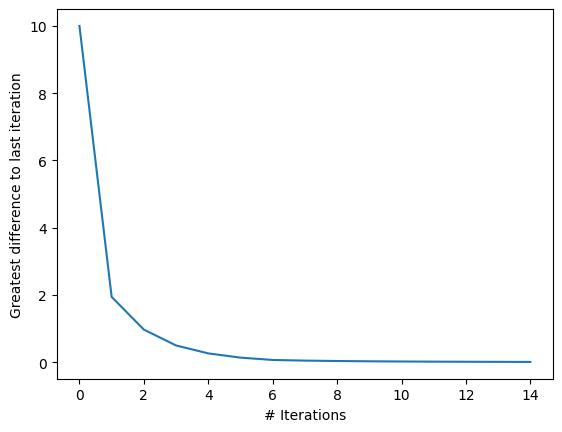
\includegraphics[width=0.75\textwidth]{img/img_2_1_a1.png}
    \caption{Konvergenzverhalten der State Values}
    \label{img:2_1_a1}
\end{figure}
Die Endwerte des Algorithmus sind in Abbildung \ref{img:2_1_a2_it15} dargestellt. Zu sehen ist dort, dass die speziellen Zellen $A$ und $B$ (Position $(0,1)$ und $(0,3)$) einen besonders hohen Wert haben. Dieser kommt dadurch zustande, dass eine Bewegung in diesen Zuständen zu einem direkten Reward von $10$ bzw. $5$ führt. Zu sehen ist jedoch auch, dass der Wert der Zustände etwas unter dem Reward-Wert liegt. Dies liegt an der Betrachtung der Folgezusstände $A'$ und $B'$, die eine negative State Value besitzen, da sie nah am Rand und zudem weit weg von $A$ und $B$ liegen, was die einzigen Zellen sind, in denen ein Übergang einen positiven Reward ungleich Null gibt. Zu sehen ist außerdem, dass aus diesem Grund die State Values höher werden, je weiter man sich den Zuständen $A$ und $B$ nähert. Um dies in Worte zu fassen: Die Zustände werden wertvoller, je näher sie an $A$ oder $B$ sind, da es dort einen hohen Reward gibt.\\
\begin{figure}
    \centering
    \begin{subfigure}[b]{0.49\textwidth}
        \centering
        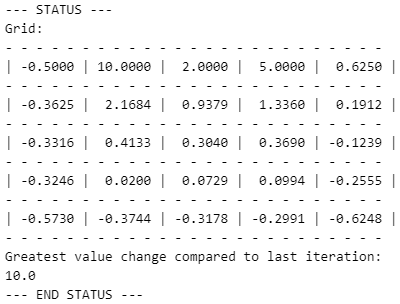
\includegraphics[width=\textwidth]{img/img_2_1_a_it1.png}
        \caption{State values nach einer Iteration}
        \label{img:2_1_a2_it1}
    \end{subfigure}
    \hfill
    \begin{subfigure}[b]{0.49\textwidth}
        \centering
        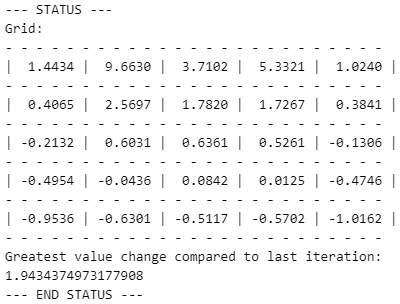
\includegraphics[width=\textwidth]{img/img_2_1_a_it2.png}
        \caption{State values nach zwei Iterationen}
        \label{img:2_1_a2_it2}
    \end{subfigure}
    \hfill
    \begin{subfigure}[b]{0.49\textwidth}
        \centering
        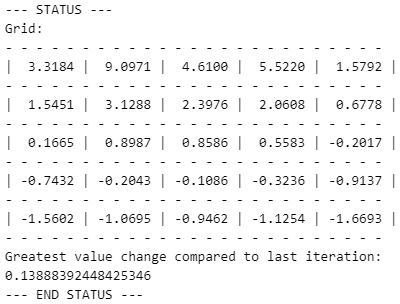
\includegraphics[width=\textwidth]{img/img_2_1_a_it5.png}
        \caption{State values nach fünf Iterationen}
        \label{img:2_1_a2_it5}
    \end{subfigure}
    \hfill
    \begin{subfigure}[b]{0.49\textwidth}
        \centering
        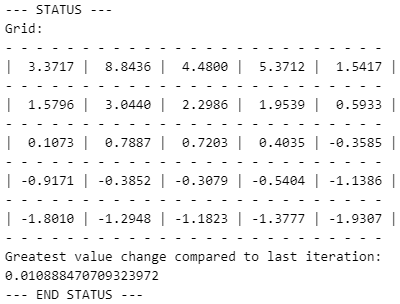
\includegraphics[width=\textwidth]{img/img_2_1_a_it_final.png}
        \caption{Endwerte der State Values (15 Iterationen)}
        \label{img:2_1_a2_it15}
    \end{subfigure}
    \caption{State Values zur Betrachtung des Konvergenzverhaltens des Algorithmus}
    \label{img:2_1_a2}
\end{figure}
Zuletzt gilt es, den Einfluss der Random-Policy zu beschreiben. Diese führt dazu, dass in jedem Zustand eine zufällige Aktion ausgeführt wird (Rechts, Links, Hoch, Runter), unabhängig von den State oder Action Values (nächstes Kapitel). Das führt dazu, dass Zelle (0,0) (oben links) einen vergleichsweise niedrigen Wert hat, obwohl sie nur einen Schritt von der Zelle mit dem höchsten Wert ($A$) entfernt ist. Dies liegt daran, dass von dort aus nur in $25\%$ der Fälle nach $A$ gewechselt wird. In $50\%$ der Fälle gibt es sogar einen negativen Reward, weil das Spielfeld verlassen wurde. Die Random-Policy führt also dazu, dass viele State Values geringer sind, als sie sein könnten, da in $50\%-75\%$ der Fälle (abhängig von der Zelle) eine nicht optimale Aktion gewählt wird.

\subsubsection*{b)}

\section*{Aufgabe 2.2}

Im folgenden werden vier Aktionen simuliert, $X$ zeigt dabei die aktuelle Position im grid an.
In diesen vier Schritten entsteht ein Gesamtreward von $0$, da weder das grid verlassen, noch $A$ oder $B$ erreicht wird.

\begin{figure}[h]
    \centering
    \begin{subfigure}[b]{0.45\textwidth}
        \centering
        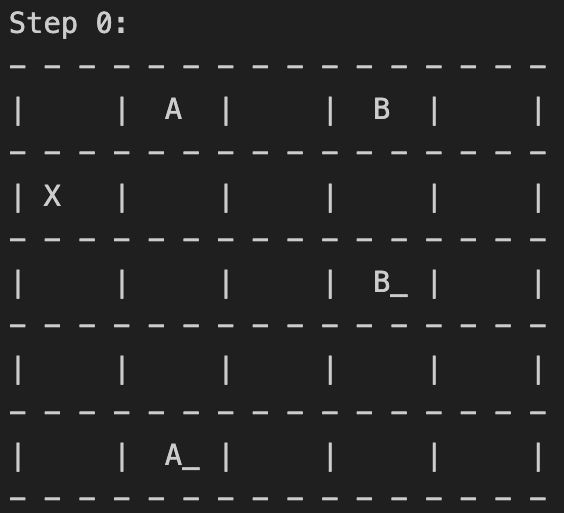
\includegraphics[width=\textwidth]{img/step_0.png}
    \end{subfigure}
    \hfill % Abstand zwischen den Bildern
    % Zweites Bild oben rechts
    \begin{subfigure}[b]{0.45\textwidth}
        \centering
        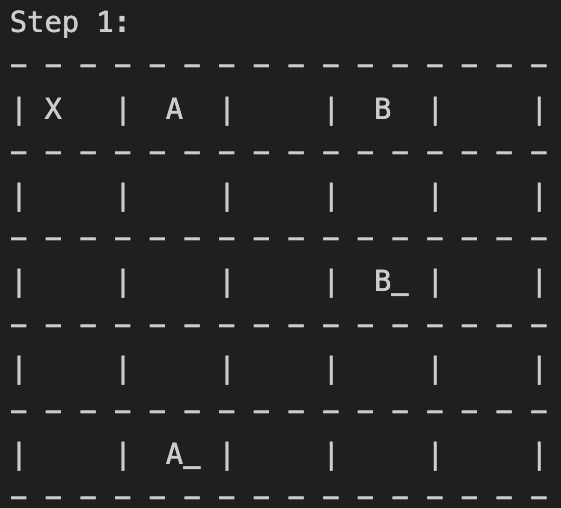
\includegraphics[width=\textwidth]{img/step_1.png}
    \end{subfigure}
    
    \vspace{1em} % Vertikaler Abstand zwischen den Zeilen
    
    % Drittes Bild unten links
    \begin{subfigure}[b]{0.45\textwidth}
        \centering
        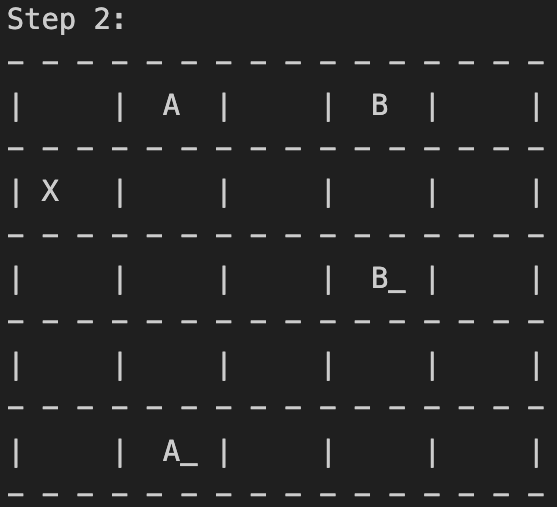
\includegraphics[width=\textwidth]{img/step_2.png}
    \end{subfigure}
    \hfill % Abstand zwischen den Bildern
    % Viertes Bild unten rechts
    \begin{subfigure}[b]{0.45\textwidth}
        \centering
        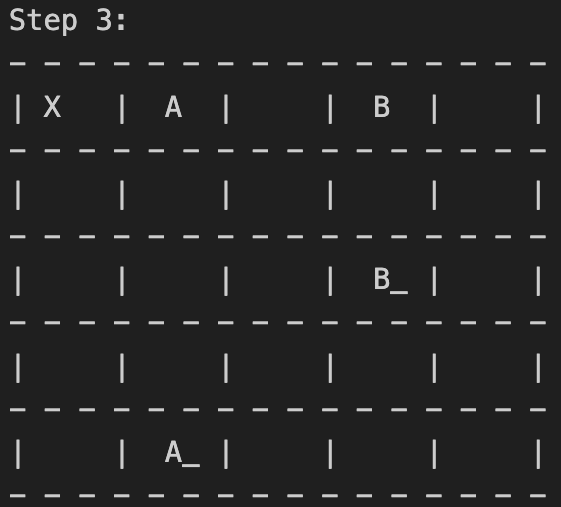
\includegraphics[width=\textwidth]{img/step_3.png}
    \end{subfigure}
\end{figure}


\section*{Aufgabe 2.3}
\subsection*{a)}
Die Menge der States $\mathcal{S}$ wird definiert durch:
\[ % enter display math mode
\begin{Bmatrix}
    \left.
    \begin{pmatrix}
        c_{xy}\\
        c_v\\
        p_\alpha\\
        p_\omega
    \end{pmatrix}
    \right\vert
    c_{xy} = Cart~position,~c_v = cart~velocity,~p_\alpha = pole~angle,~p_\omega = angular~velocity~of~pole
\end{Bmatrix}
\]%  
Das heißt, dass ein konkreter Zustand durch die Kombination der Cart-Position, -Geschwindigkeit, der Pole-Position und der Pole-Winkelgeschwindigkeit definiert wird.\\
Die Aktionen $\mathcal{A}$ sind gegeben durch:
\[ % enter display math mode
\begin{Bmatrix}
    Cart~nach~links~schieben, && Cart~nach~rechts~schieben
\end{Bmatrix}
\]% 
Die Zustandsübergänge werden dabei durch die Bewegungsgleichungen der physikalischen Umgebung definiert. So kann eine Cart-Bewegung nach links den Pole, abhängig von der Cart- und Pole-Geschwindigkeit, nach links fallen lassen, die Fallgeschwindigkeit verringern oder gar einen Fall nach rechts veranlassen oder diesen beschleunigen. Analog für eine Cart-Bewegung nach rechts.\\
Die Belohnungsstruktur hängt davon ab, was das endgültige Ziel ist. Sofern das Ziel ``nur'' ist, den Pole nicht fallen zu lasen, kann man alle Zustände, in denen die Umgebund nicht endet, mit einem einheitlichen Reward (beispielsweise $1$ oder $0$) versehen. Die Zustände, in denen der Pole umfällt und die Umgebung somit endet, kann man mit einem negativen Reward (wie beispielsweise $-1$) ``bestrafen''. Falls das Ziel jedoch darin besteht, den Poly in einer bestimmten Position zu behalten, könnten die Zustände mit der gewünschten Position mit einem hohen Reward belohnt werden, der mit der Abweichung vom gewünschten Zustand abnimmt.\\
Da keine genaueren Vorgaben gemacht werden und es üblich ist, das reine ``Überleben'' des Poles zu belohnen, wird folgende Belohnungsstruktur zugrunde gelegt: $0$ für alle Übergänge zu Zustanden, in denen die Umgebung endet, $+1$ zu allen Zuständen, in denen die Umgebung nicht endet. \\
Eine Simulation mit einer zufälligen Aktionswahl ist im beiliegenden Jupyter-Notebook dargestellt und dient nur dazu, ein Gefühl dafür zu bekommen, wie sich das Environment verhält.

\subsubsection*{b)}

Um das CartPole-Problem zu lösen (den Pole möglichst lange aufrecht halten und nicht aus dem Environment herausfahren), wurden zunächst drei Policies betrachtet und simuliert, die ohne Learning-Ansätze auskommen.\\
\textbf{Policy 1:} Die erste Policy ist besonders simpel. Sie kontert die Neigung des Poles, indem sie das Cart in die Richtung bewegt, in die der Pole aktuell geneigt ist.\\
\textbf{Policy 2:} Die zweite Policy stellt die erste iterative Erweiterung/Verbesserung der Policies dar. Neben der Pole-Position wird nun auch die Winkelgeschwindigkeit betrachtet. Nun wird nicht mehr einfach versucht, den Winkel des Poles zu ``kontern'', sondern auch den Fall zu verhindern. Das heißt, wenn der Pole nach  links fällt, bewegt sich auch das Cart nach links. Wenn der Pole nach rechts fällt, fährt das Cart auch nach rechts. Dabei inkludiert ein ``Fall nach rechts'' auch die Situation, in der der Pole zwar einen negativen Winkel aber eine positive Winkelgeschwindigkeit hat. Das Ziel ist, eine Überkorrektur zu vermeiden und den Fall des Poles wieder abzubremsen.\\
\textbf{Policy 3:} Die dritte Policy baut auf der zweiten auf, indem das Cart aktiv vom Rand des Environments ferngehalten wird. Das heißt, wenn das Cart sich auf eine bestimmte Distanz dem linken Rand nähert, wird es nach rechts bewegt. Analog für den rechten Rand. Dadurch achtet die dritte Policy darauf, beide Bedingungen, die zu einem Episodenende führen können, zu vermeiden: Das Umfallen des Poles und das Herausfahren des Carts.\\
Die Ergebnisse der Policies sind in Abbildung \ref{img:2_3_b} zu sehen.

\begin{figure}
    \centering
    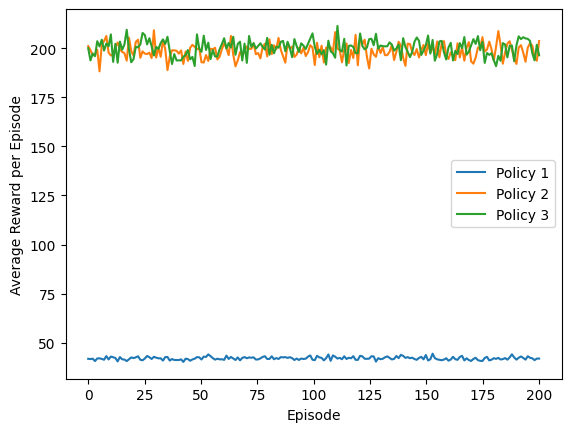
\includegraphics[width=\textwidth]{img/img_2_3_b.png}
    \caption{Policy-basierte Simulation des CartPole Environments ohne Learning-Ansätze. 100 Durchläufe (1 Durchlauf = 200 Episoden) zur Mittelung der Werte.}
    \label{img:2_3_b}
\end{figure}

Zunächst gilt es, die Effektivität der Policies zu beurteilen. Abbildung \ref{img:2_3_b} suggeriert starke Unterschiede zwischen Policy 1 und den beiden Erweiterungsstufen. Das heißt, dass ein Betrachten der Winkelgeschwindigkeit des Poles, um eine Überkorrektur der Position zu vermeiden, einen signifikanten Einfluss auf die Performance eines Ansatzes hat. Der Unterschied zwischen Policy 2 und 3 ist hingegen nur sehr klein. Policy 3 zeigt jedoch meist eine marginal bessere Performance. Das heißt, dass ein reines ``Weglenken'' vom Rand, ohne die Pole-Position zusätzlich zu beachten, nur zu einer minimal längeren Simulationszeit führt. Dies kann daran liegen, dass der Pole in einem der nächsten Schritte umfällt, da das Cart eigentlich noch weiter in Richtung des Randes fahren müsste, um die Pole-Bewegung auszugleichen.\\
Die Schwierigkeit liegt also darin, die optimale Handlung für alle Kombinationen aus Pole- und Cart-Status zu finden. Besonders die Situationen, in denen ein feinfühliges Handeln notwendig ist (langsames Wegfahren vom Rand ohne den Pole zu stark auszulenken), stellen ein Problem für die Policy dar, da sie nur wenige grundlegende Fallunterscheidungen machen.\\
Abbildung \ref{img:2_3_b} zeigt außerdem eindrücklich die Stabilität der Policies (Stabilität meint dabei die Konstanz des Ergebnisses). Zu sehen ist, dass der durchschnittliche Reward der einzelnen Policies über alle Episoden hinweg annähern gleich bleibt. Insgesamt wurden $100$ Durchgänge durchgeführt, wobei ein Durchgang aus $200$ Episoden besteht. Das heißt, dass sich der Reward-Wert pro Episode als Durchschnitt aus $100$ Werten berechnet. Die hohe Stabilität der Policies zeigt, dass sie nicht auf ``glückliche Zufälle'' angewiesen sind oder nur aufgrund unglücklicher Umstände einen niedrigen Reward pro Episode erreichen.\\
Die Zielerreichung lässt sich aus zwei Sichten auf den Begriff ``Ziel'' analysieren: 1. Das Ziel ist, aufgrund der Veränderungen zwischen den Policy-Versionen einen besseren Reward zu erzielen oder 2. Das Ziel ist, einen möglichst hohen Reward zu erzielen. Die erste Definition des Begriffs ``Ziel'' wurde zuvor bereits im Zuge der Effektivität analysiert. Zusammenfassend lässt sich hier dementsprechend noch einmal erwähnen, dass die Veränderungen zwischen den Policies zu einer stetigen Erhöhung des durchschnittlichen Rewards führen. Vor allem die Veränderung des Rewards von Policy 1 zu Policy 2 ist signifikant hervorzuheben. Mit Hinblick auf die zweite Definition des Begriffs ``Ziel'' sollte man zuvor definieren, was der maximal erreichbare Reward ist. Dieser liegt laut Dokumentation bei $500$. Das heißt, dass Policy 1 nicht einmal $10\%$ des maximalen Rewards erreicht. Policy 2 und 3 liegen immerhin bei etwa $40\%$. Das legt jedoch nahe, dass noch Raum für Verbesserung besteht und keine der oben vorgestellten Policies ausreicht, um die Umgebung dauerhaft in einer stabilen Situation zu behalten. Stabil meint dabei: Den Pole aufrecht und stationär und das Cart möglichst nah in der Mitte und ebenfalls stationär. 

\subsubsection*{c)}
% TODO: Effektivität des Ansatzes Diskutieren (Performance + Konvergenzverhalten)
% TODO: Effizienz der Diskretisierung diskutieren
Ziel ist es, mithilfe einer Diskretisierung der Beobachtungszustände den Environments einen Reinforcement-Learning Ansatz mithilfe der bereits bekannten ``Banditen'' zu implementieren. Der zugehörige Code ist dem beiliegenden Notebook zu entnehmen.
Für die Diskretisierung wurden folgende Zustände gewählt:
\begin{enumerate}
    \item Negativer Pole-Winkel, negative Pole-Geschwindigkeit 
    \item Negativer Pole-Winkel, positive Pole-Geschwindigkeit 
    \item Positiver Pole-Winkel, negative Pole-Geschwindigkeit 
    \item Positiver Pole-Winkel, positive Pole-Geschwindigkeit 
\end{enumerate}
Für diese Diskretisierung wurde sich entschieden, da der Policy-basierte Ansatz für die Betrachtung dieser Informationen bereits vielversprechende Ergebnisse gezeigt hat und dieser ``einfache'' Fall verhältnismäßig einfach auszuwerten ist, um Informationen für Verbesserungen und Erweiterungen zu erhalten. Dies wird im späteren Verlauf dieses Abschnitts diskutiert.\\
\begin{figure}
    \centering
    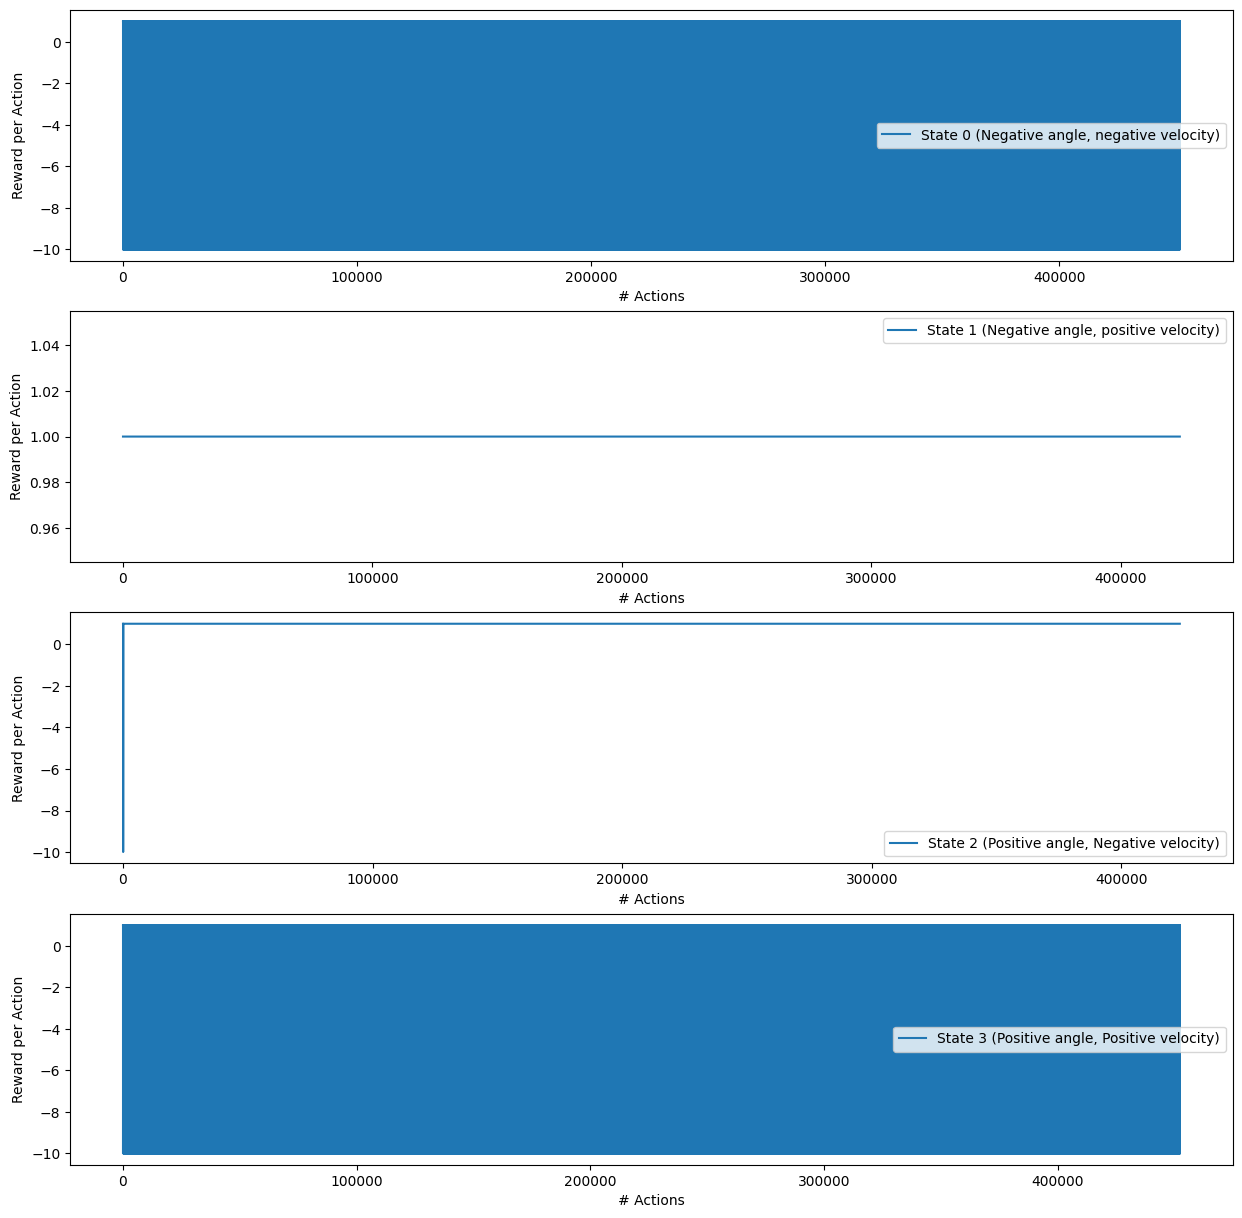
\includegraphics[width=\textwidth]{img/img_2_3_c1.png}
    \caption{Reward pro gewählter Aktion für jeden Banditen (Label ``angle'' und ``velocity'' beziehen sich je auf Pole-Position und -Winkelgeschwindigkeit)
    \label{img:2_3_c1}}
\end{figure}
Zunächst gilt es, die Effektivität dieses Ansatzes zu beurteilen. Um dies zu tun, sind Abbildung \ref{img:2_3_c1} und Abbildung \ref{img:2_3_c2} zusammen zu betrachten. In Abbildung \ref{img:2_3_c1} ist zu sehen, dass vor allem Zustand 0 und 3, das sind die Zustände, in denen der Pole umzufallen droht, auch nach $400.000$ Aktionen keinen stationären Endwert annehmen. Es wird also nicht durchgehend positiver Reward gesammelt. Dass der Graph der beiden Zustände einer blauen Fläche ähnelt, liegt daran, dass er schnell zwischen $1$ und $-10$ wechselt. Durch die Linienbreite führt dies zur blauen fläche. Der ständige Wechsel des Rewards kann bedeuten, dass eine Aktion, die früh im Umfall-Prozess stattfindet, nicht zur Terminierung der Episode führt, einen Zeitschritt später hingegen schon. Dies ist ein Indiz für eine suboptimale Wahl der Diskretisierung, dies wird jedoch gleich erst näher erläutert. Zustände 1 und 2 konvergieren hingegen, zumindest hinsichtlich des Rewards. Das kann daran liegen, dass der Pole gerade sowieso ``gerettet'' wird, das heißt er bewegt sich in Richtung der aufrechten Position. In diesem Zustand spielt es keine so große Rolle, welche Aktion durchgeführt wird, da es ein verhältnismäßig sicherer Zustand ist, der nicht zu einem direkten Umfallen des Poles führen kann. Hinsichtlich der Aktionen konvergiert der Bandit hier jedoch mit geringer Wahrscheinlichkeit, da keine der Aktionen die offensichlich bessere oder schlechtere ist. Beide scheinen gleich gut.\\
\begin{figure}
    \centering
    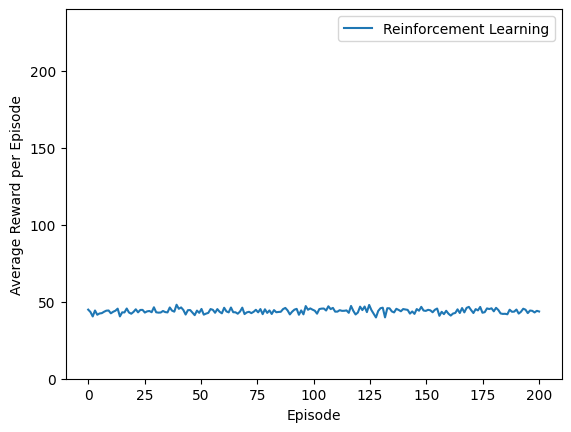
\includegraphics[width=\textwidth]{img/img_2_3_c2.png}
    \caption{Reinforcement Learning basierte Simulation des Environments. 100 Durchläufe (1 Durchlauf = 200 Episoden) zur Mittelung der Werte.}
    \label{img:2_3_c2}
\end{figure}
Um nun die Performance zu untersuchen, ist Abbildung \ref{img:2_3_c2} hilfreich, da sich diese direkt mit Abbildung \ref{img:2_3_b} vergleichen lässt. Zu sehen ist, dass der Learning-basierte Ansatz im Schnitt nur einen Reward von etwa $50$ erhält und damit nur $10\%$ des theoretischen Maximalwertes. Und das obwohl dieser Ansatz grundsätzlich die gleichen Informationen verwendet wie Policy 2 in Abbildung \ref{img:2_3_b}. \\
Die Gründe dafür können in der Diskretisierung liegen. In diesem Fall wurden die Zustände sehr grob gewählt. Das heißt, es wird nur Unterschieden zwischen ``Pole nach links geneigt'' und ``Pole nach rechts geneigt'' (Analog für die Winkelgeschwindigkeit), nicht jedoch wie weit der Pole jeweils geneigt ist. Das führt dazu, dass ein nach links fahren bei nach links geneigtem Pole bei einem kleinen Winkel noch in Ordnung sein kann, im nächsten Zeitschritt jedoch zum Umfallen führt. Dadurch ist es schwierig für den Banditen herauszufinden, was die beste Option ist. Das Problem kann auch damit zusammenhängen, dass der Bandit nicht in die Zukunft schaut. Er betrachtet nur den direkten Reward, nicht jedoch, wie sich seine Aktion auf die zukünftigen Zustände auswirkt. Dadurch kann es eben dazu kommen, dass der Bandit den Pole in eine noch ungünstigere Position bringt, solange die Episode nicht terminiert.\\
Hilfreich wäre also eine feinere Diskretisierung der Zustände, um zwischen ``Pole ist leicht geneigt'' und ``Pole droht umzufallen'' zu unterscheiden. Außerdem könnte es sinnvoll sein, die Cart-Informationen mit einzubeziehen, um ein ``Herausfahren'' des Carts aus der Szene zu verhindern. Dies wurde im oben genannten Ansatz nicht beachtet und kann auch ein Grund für den niedrigen Reward sein. Ein Problem, das auch eine feinere Diskretisierung nicht verhindern kann, ist das fehlende Zukunftsbewusstsein des Algorithmus. Also, dass der Algorithmus vermeidet, den Pole in eine schlechtere Ausgangsposition für den nächsten Zeitschritt zu bringen, auch wenn es im aktuellen Zeitschritt nicht zur direkten Terminierung führt. 

\end{document}